% ====================================================================
%+
% SECTION:
%    MW_FutureWork.tex
%
% CHAPTER:
%    galaxy.tex
%
% ELEVATOR PITCH:
%    Ideas for future metric investigation, with quantitaive analysis
%    still pending.
%-
% ====================================================================

\section{Future Work}
\def\secname{MW_future}\label{sec:\secname}

In this section we provide a short compendium of science cases that
are either still being developed, or that are deserving of quantitative
MAF analysis at some point in the future.

% ====================================================================

% % ====================================================================
%+
% SECTION:
%    section-name.tex  % eg lenstimedelays.tex
%
% CHAPTER:
%    chapter.tex  % eg cosmology.tex
%
% ELEVATOR PITCH:
%    Explain in a few sentences what the relevant discovery or
%    measurement is going to be discussed, and what will be important
%    about it. This is for the browsing reader to get a quick feel
%    for what this section is about.
%
% COMMENTS:
%
%
% BUGS:
%
%
% AUTHORS:
%    Phil Marshall (@drphilmarshall)  - put your name and GitHub username here!
%-
% ====================================================================

\section{Dust in the Milky Way}
\def\secname{MW_Dust}\label{sec:\secname} % For example, replace "keyword" with "lenstimedelays"

\noindent{\it Peregrine M. McGehee} % (Writing team)

% This individual section will need to describe the particular
% discoveries and measurements that are being targeted in this section's
% science case. It will be helpful to think of a ``science case" as a
% ``science project" that the authors {\it actually plan to do}. Then,
% the sections can follow the tried and tested format of an observing
% proposal: a brief description of the investigation, with references,
% followed by a technical feasibility piece. This latter part will need
% to be quantified using the MAF framework, via a set of metrics that
% need to be computed for any given observing strategy to quantify its
% impact on the described science case. Ideally, these metrics would be
% combined in a well-motivated figure of merit. The section can conclude
% with a discussion of any risks that have been identified, and how
% these could be mitigated.

Interstellar dust is a significant constituent of the Galaxy. Its composition and associated extinction
properties tell us about the material and environments in which stars and their planets are formed.
Dust also presents an obstacle for a wide-range of astronomical observations, causing light from
stars in the plane of the Milky Way to be severely dimmed and causing the apparent colors of
objects observed in any direction to be shifted from their intrinsic values. These color shifts
are dependent upon the dust column density along the line of sight and the radiative transport
properties of the dust grains.

The wavelength dependence of the absorption due to dust is parametrized in the widely used model
of Cardelli et al. (1989) by the ratio of general to selection extinction in the Johnson B and V
bands, defined as RV = AV /E(B − V ). The value of RV depends on the dust composition and
grain size along the line of sight. In the low-density diffuse ISM, RV has a value ∼ 3.1, while in
dense molecular clouds, RV can be higher with values 4 < RV < 6.

The fundamental importance of a well-characterized dust map to astronomy is underscored by the
> 5, 000 citations to the dust and extinction maps by Schlegel et al. (1998), henceforth SFD98.
The SFD98 maps are based on far-infrared observations and predict reddening in specific bands by
assuming a dust model and RV = 3.1 as appropriate for sky areas away from the Galactic plane.
Despite the great contribution that the SFD98 extinction map has made to the field, these maps
suffer from several issues that limit their utility in some regimes of study. 1) While the SFD98
map seems to be well calibrated at low column density, various tests using galaxy counts, star
counts and colors, and stellar spectrophotometry indicate that SFD98 overpredicts dust by ∼ 30%
above E(B − V ) ∼ 1 mag. Because this overcorrection appears especially in cold clouds, it is
likely related to the temperature correction adopted in the SFD98 model. 2) In some cases,
especially at low Galactic latitudes, RV variation is important and is not tracked by SFD98. 3)
For study of low-redshift, large-scale structure, contamination by unresolved point sources can be
important (see Yahata et al. 2007). 4) Finally, the resolution of the SFD98 map is ∼ 60, which
is larger than the angular scales subtended by nearby, resolved, galaxies for which a carefully
characterized foreground dust distribution is particularly important. For all these reasons, LSST
stellar photometry, which can constrain the temperature correction, overall calibration, and point
source contamination of SFD98, is valuable.

For the study of stellar populations and objects within the Galactic disk it is also important to
determine both the line of sight extinction and the value of RV at a specific distance, neither of
which is dealt with by SFD98. By analysis of the observed reddening of stellar colors, we will verify
both the dust column density and RV values predicted by these maps and can also determine the
local spatial distribution of the dust. We will do this utilizing two specific stellar populations - the
M dwarfs and the F turn-off stars.

The reddening of stellar colors due to the presence of interstellar dust along the line of sight can,
in principle, be used to map the three-dimensional distribution of that dust. This requires that
two important parameters are determined - the amount the observed stellar color is reddened and
the distance to the star. By comparison of the color excess measured in stars at varying distances
we can infer the location of the extincting medium. However, given lack of an a priori knowledge
of the light of sight extinction, which is the very quantity we wish to measure, it can be difficult
to accurately assign intrinsic stellar colors and luminosities in order to determine the amount of
color excess and the distance. This difficulty can be surmounted, however, if we utilize reddeninginvariant
combinations of colors whose values can be used to infer location on the stellar locus
and hence intrinsic colors and luminosities. This technique is viable if we use LSST photometry of
M dwarfs as the stellar locus in ugriz colors is nearly parallel to the reddening vector for all but
coolest stars.


% --------------------------------------------------------------------

\subsection{Target measurements and discoveries}
\label{sec:\secname:targets}

The use of stellar samples to create three-dimensional extinction maps has an established history
beginning with the work of Neckel & Klare (1980); however these, including studies based on SDSS
photometry, are typically limited to heliocentric distances of 1−2 kpc. In the full co-added survey,
LSST will be able to map dust structures out to distances exceeding 15 kpc, thus revealing a
detailed picture of this component of the Milky Way Galaxy.

Mapping of the dust component of the Galactic ISM requires detection of the reddening in the
colors of stars at known distances. The reddening is determined from the color excess deduced
by comparison of the observed colors with those expected based on the stellar spectral type. In
the absence of identifying spectra, the spectral type can be inferred by dereddening the observed
colors (assuming a specific extinction law, i.e., a particular value of RV ) back to the unreddened
stellar locus in a color-color diagram. This dereddening is equivalent to assignment of reddeningfree
colors along the stellar locus, which measure the location in the color-color diagram along
the direction perpendicular to the reddening vector. Once the effective line of sight reddening has
been computed, the distance to each star can be determined using dereddened photometry and
well-calibrated color-absolute magnitude relations.


Reddening-invariant Indices

Reddening-free colors were defined in the SDSS ugriz system by McGehee et al. (2005) for characterization
of embedded pre-main sequence stars and were subsequently used as part of the SDSS
photometric quality analysis system (Abazajian et al. 2009). The general definition is
Qxyz = (x − y) − (y − z) ×
E(x − y)
E(y − z)
(7.1)
where (x − y) and (y − z) are the colors used to construct the color-color diagram. This extends
the definition by Johnson & Morgan (1953) whose original Q would be defined here as QUBV . The
reddening coefficients adopted by the SDSS (Stoughton et al. 2002) follow SFD98 and assume the
“standard” dust law of RV = 3.1 and a z = 0 elliptical galaxy spectral energy distribution.
In Figure 7.4 we compare the variation of the three reddening-invariant indices formed from the
ugriz passbands (Qugr, Qgri, and Qriz) with g − i, a proxy for stellar spectral type (Covey et al.
2007). For g − i < 1.9 (spectral type earlier than M0) there is little variation in any of these
indices, indicating that the stellar locus is approximately parallel to the reddening vector in the
corresponding color-color diagrams. For the M dwarfs we see that the Qgri has the largest range
between M0 and M5, and thus is of the greatest utility for determination of spectral type.
213

Selection of Reddening Probes

For determination of spectral type and intrinsic stellar colors to be accurate, the stars used as
reddening probes must reside on the portion of the stellar locus that is not aligned with the
reddening vector in a color-color diagram. As we have seen, this condition is fulfilled by stars of
spectral types M0 and later. In the final panel of Figure 7.4 we show the criteria used to select
for early and mid M dwarfs based on the Qgri and Qriz indices, where the latter is used to filter
out earlier and more luminous background stars whose Qgri colors are similar to M0 dwarfs. The
threshold at M5 is chosen to remove the later spectral type stars, which are too intrinsically faint
to serve as probes for all but the nearest dust structures.

Analysis of the LSST imaging data will adapt the following procedure as used in the SDSS High
Latitude Cloud Survey (McGehee 2009):
• The intrinsic g − i color ((g − i)0) is determined from the observed Qgri color based on a
fifth-order polynomial fit using the median stellar locus (Covey et al. 2007) and assuming
RV = 3.1.
• The total reddening to each star is computed from the g − i color excess.
• Distances are assigned based on the color-absolute magnitude relations of Ivezi´c et al. (2008)
using the dereddened photometry.
• E(B − V ) maps are created at specific distance ranges using the adaptive technique of
Cambr´esy et al. (2005) in which the reddening at each pixel is the median of that computed
for the N nearest extinction probes.

Example maps from the SDSS project are depicted in Figure 7.5 for a 10◦ by 10◦ field containing the
high latitude molecular cloud HRK 236+39. These maps are based on the reddening computed for
stars having distance moduli of 7.0 < m − M < 8.0, 8.0 < m − M < 9.0, and 9.0 < m − M < 10.0.
The reddening shown at each pixel is computed as the median of the E(B − V ) values obtained
for the N = 5 nearest stars. The reddening associated with the HRK 236+39 cloud is discernible
at m − M > 7.0 (d > 250 pc) and is obvious at m − M > 8.0 (d > 400 pc).

Distance and AV Limits

It has been demonstrated that accurate three-dimensional mapping of the local ISM within a few
kpc is possible using SDSS photometry of M dwarfs (McGehee 2009). Analysis of the g − i color
excess in regions effectively free of interstellar reddening shows that distance modulus limits of 7.0
(at M5) to 11.2 (at M0) result in a volume-limited survey nearly free of the systematic color biases
inherent in this g-band limited data set.

These limits correspond to g ∼ 20.6 and σg ∼ 0.02−0.03 for single-epoch SDSS observations. Given
the relative g-band 5 σ limits of SDSS and the LSST single epoch and final co-added surveys, we
estimate that the the co-added LSST data will reach 5 magnitudes deeper in m-M, allowing the
LSST to probe dust structures across a significant portion of the Galaxy. In Figure 7.6 we depict
the portion of the Galactic disk accessible by the LSST single and co-added surveys as well as the
SDSS assuming the vertical and radial scale height dust model outlined in § 3.7.1.

7.5.2 Variation in Extinction Laws

Changes in the absorption properties of dust grains, as parametrized by RV , result in a shift in
both the direction and length (for a specific dust column density) of the reddening vector in a
color-color diagram. This is reflected in the reddening-free colors by variations in the scaling factor
used when defining the linear combination of colors, e.g., in the E(g − r)/E(r − i) term for Qgri.
By analysis of the observed color shifts due to reddening it is possible to constrain the value of RV
along the line of sight and gain insight into the nature and composition of the interstellar dust in
that region of the Galaxy.

The LSST will be in a unique position to measure the changes in the observed reddening vector
due to RV variations due to its superb photometric accuracy (see § 2.6). The specifications for
LSST are a factor of two more stringent than typically achieved in previous surveys, including the
SDSS (except for limited photometric conditions).

F turn-off stars (gabs ∼ 4) reside on the blue tip of the stellar locus in ugriz color space and for
g > 19 trace the total Galactic extinction along high-latitude lines of sight. This method will
provide a verification of the far-infrared-based SFD98 extinction model and allow study of the
variations in dust grain sizes as inferred from RV . The value of RV provides a general indicator of
grain size, with the RV ∼ 4.5 − 5 values seen in star formation regions suggestive of grain growth
in cold molecular clouds.

The slope of the reddening vector is sensitive to the value of RV as shown in Figure 7.7. For the
SDSS passbands and an assumed F star source SED, the value of E(u−g)/E(g−r) is larger for small
RV and decreases with a slope of approximately −0.11 with increasing RV . This analysis mandates
precise and well-calibrated photometry. For example, determination of RV to within σRV = 0.5
requires the slope of the reddening vector to be measured to σm = 0.06. If E(B −V ) = 1 along the
line of sight, then the required photometric accuracy is 2%. The photometric accuracy requirement
becomes proportionally more stringent as the dust column density decreases due to the reduced
movement of the blue tip in the color-color diagram. LSST, with better than 1% photometric
accuracy in the final co-added survey, will be able to study RV variations in both Galactic plane
and high latitude environments.
Describe the discoveries and measurements you want to make.

Now, describe their response to the observing strategy. Qualitatively,
how will the science project be affected by the observing schedule and
conditions? In broad terms, how would we expect the observing strategy
to be optimized for this science?


% --------------------------------------------------------------------

\subsection{Metrics}
\label{sec:\secname:metrics}
 From the material in the science book and what you have contributed, I think a metric dependent on the photometric accuracy metrics might be the way to go (e.g. estimate the error in A_V and E(B-V) for different strategies, which would be a simple scaling for each pixel in the spatial map given the nominal scalings with exposure time in each filter).

The spacing in time of the visits doesn't matter for dust (as far as I know). 
Pushing to fainter magnitudes (which means both better seeing and longer exposures) matters, both because we want more stars, and in particular, we want more stars *behind* the dust.  If we can't see through the dust, we can't do much.  At PS1 depth, we get to ~ 3-5 kpc, with maybe up to 1ish mag E(B-V).  If we went 3 or 4 mags fainter, how far could we go?  This is a good question, and one I am unlikely to answer by next week.  But it is something we should figure out. 

I'm cc'ing Greg in case he has a better answer, or in case he has some mock map runs that give us an idea of how our results depend on survey depth. 
Quantifying the response via MAF metrics: definition of the metrics,
and any derived overall figure of merit.

{\bf Metric 1: Uncertainty and bias in $E(B-V)$~estimates as a
  function of location on-sky.} Dependencies:

\begin{itemize}
  \item Stellar population throughout the survey (e.g. Knut / Peter developments; TRILEGAL?);
    \item Dust map throughout the survey region;
    \item Scale photometric error predictions for each band from program requirements per exposure;
      \item Produce formal estimate on the error in extinction and reddening as a function of position on-sky within the survey.
\end{itemize}


% --------------------------------------------------------------------

\subsection{OpSim Analysis}
\label{sec:\secname:analysis}

OpSim analysis: how good would the default observing strategy be, at
the time of writing for this science project?


% --------------------------------------------------------------------

\subsection{Discussion}
\label{sec:\secname:discussion}

Discussion: what risks have been identified? What suggestions could be
made to improve this science project's figure of merit, and mitigate
the identified risks?


% ====================================================================

\navigationbar


% ====================================================================

% WIC - promoted this back to MW Halo section

% % ====================================================================
%+
% SECTION:
%    section-name.tex  % eg lenstimedelays.tex
%
% CHAPTER:
%    chapter.tex  % eg cosmology.tex
%
% ELEVATOR PITCH:
%    Explain in a few sentences what the relevant discovery or
%    measurement is going to be discussed, and what will be important
%    about it. This is for the browsing reader to get a quick feel
%    for what this section is about.
%
% COMMENTS:
%
%
% BUGS:
%
%
% AUTHORS:
%    Phil Marshall (@drphilmarshall)  - put your name and GitHub username here!
%-
% ====================================================================

\section{Mapping the Milky Way Halo}
\def\secname{MW_Halo}\label{sec:\secname} % For example, replace "keyword" with "lenstimedelays"

\noindent{\it Kathy Vivas, Colin Slater, David Nidever, Beth Willman}  % (Writing team)

The study of the Halo of the Milky Way is of the most importance not only to understand
the formation and early evolution of our own galaxy, but also to test 
test current models of hierarchical galaxy formation. 
LSST will provide an unprecedented combination of
area, depth, multi-band, multi-epoch information for pursuing detail studies
of the structure of this old Galactic component. We focus here in three
specific projects that can be pursued with LSST. We suggest metrics and figure of merits that can
be calculated in order to quantify the feasibility of the projects under different
observational strategies. We expect more projects will join later.

RR Lyrae stars have been known for several decades as excellent tracers
of the halo population. They are not only old stars ($>10$ Gyrs) but they are
also excellent standard candles that allow to build 3-dimensional maps. 
The halo of the Milky Way has been now surveyed in a very large extension up to 
$\sim 60-80$ kpc from the Galactic center \citep[][among others]{drake13a,drake13b,zinn14,torrealba15}. 
Beyond that, the halo is
mostly uncharted territory.
From these RR Lyrae surveys, we have learned that the halo is filled with substructures
which are usually interpreted as debris from destroyed satellite galaxies. The smooth 
component of the RR Lyrae distribution is well described
with a power-law of the mean number density of RR Lyrae stars as a function of
galactocentric distance, which gets steeper after $\sim 30$ kpc \citep{zinn14}. 
Thus, beyond $\sim 60$ kpc, few field RR Lyrae stars are expected. However, we presume that 
any RR Lyrae star beyond this distance may be part of either debris material or distant
satellite galaxies of low luminosity that have been escaped detection until now \citep{sesar14,baker15}. 
LCDM models predict debris as far as $0.5$~Mpc from the galactic center
This is the territory that will be explored by LSST.

Similarly, red giant stars can be used to trace the structure of the halo up to large
distances. They have the advantage 
of being bright and numerous stars.

Fainter than these two tracers, main sequence stars stand up as a tool for studying
the Halo. They are the most numerous type of stars available and statistical studies 
are possible. Using the technique of photometric metallicities \citep{ivezic08}, 
SDSS provided unprecedented maps of the metallicity distribution up to  $\sim 10$ 
kpc from the Galactic center, unveiling not only the mean metallicity distribution 
of the halo but also, sub-structures within the halo. This kind of works will be extended
to the outermost parts of the Galaxy with LSST data.


% --------------------------------------------------------------------

\subsection{Target measurements and discoveries}
\label{sec:\secname:MW_Halo_targets}

The three projects just described require the discovery and/or measurement of the following 
type of objects:

\begin{itemize}

\item RR Lyrae stars: These are bright horizontal-branch variable stars with
periods between 0.2 to 1.0 days and large amplitudes, particularly in the bluer 
bandpasses (g amplitudes $0.5 - 1.5$~mag). \citet{2012AJ....144....9O} made an intensive
search for RR Lyrae stars in simulated LSST data and reached to the conclusion 
that this type of stars can be recovered to distances $\sim 600$ kpc. A similar procedure
can now be performed using MAF and current cadence scenarios.
Chapter \ref{chp:variables} discusses the discovery metrics for variable stars 
including RR Lyrae stars. However, optimal recovery may involve more complex metrics
involving the simultaneous use of multi-band time series \citep{vanderplas15,vivas16}.
Besides the recovery of the variable stars, a particularly valuable measurement to track 
for studies in the halo is the infrared mean magnitudes z and y since they provide the 
most accurate way to obtain distances \citep{caceres08}. 

\item Main sequence stars: lacking any distinguishable variability, the
challenge in selecting a large and clean sample of main sequence stars comes
from tremendous number of small and nearly-unresolved galaxies present at
faint magnitudes. Precise star/galaxy separation is thus the limiting factor
on the useful depth of the main sequence sample. In addition to identifying
dwarfs, using dwarfs to map the metallicity distribution of the halo requires
precise u-band data, since it exhibits the strongest metallicity dependence of
the LSST filters.

\item Red Giants: due to their intrinsic luminosity red giants will be sample
a far deeper volume than main sequence stars at similar apparent magnitudes,
but they must first be identified and separated from the very numerous main
sequence stars present in the field. A gravity-sensitive photometric index can
be used for separating efficiently giants from dwarfs. The u magnitude
is an essential ingredient in this process and it is necessary to follow-up
the behavior of the u limiting magnitude under different observational
strategies. Figure~\ref{fig-MW-giants} shows the distance that can be reached 
by M giants of different metallicities assuming a limiting magnitude in the u band of
26.0. 

\end{itemize}

\begin{figure}
\begin{center}
  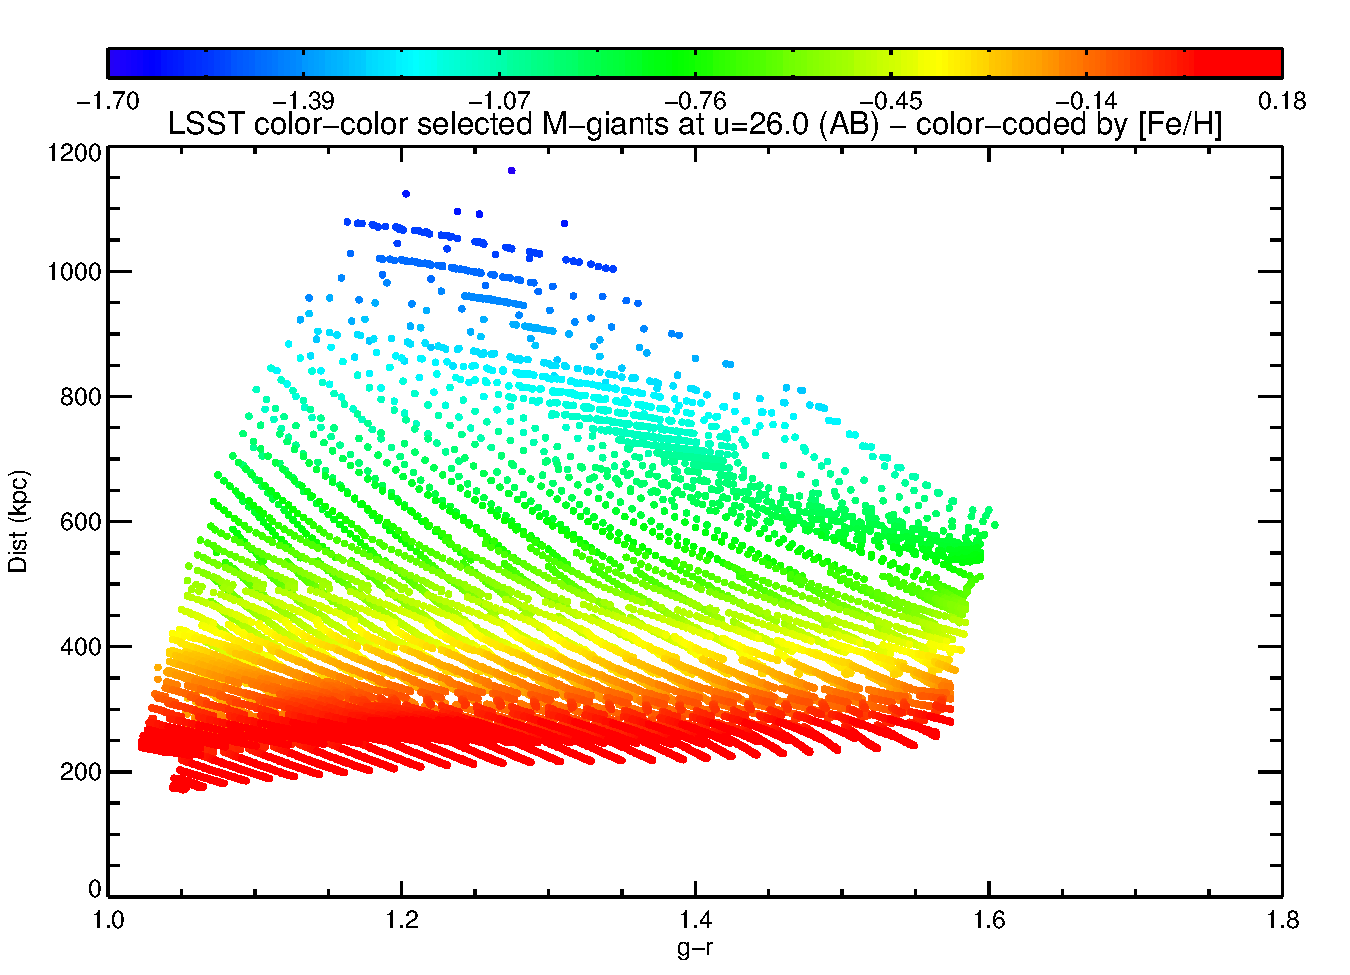
\includegraphics[scale=0.5]{./figs/milkyway/lsst_mgiants_grdist.pdf}
  \caption{Distance to which red giant stars can be identified in the galactic halo asuuming a limiting magnitude
  of u=26.0. The color code scales with the metallicity of the stars. More metal-poor stars can be 
  detected to farther distances. \label{fig-MW-giants}}
\end{center}
\end{figure}


% --------------------------------------------------------------------

\subsection{Metrics}
\label{sec:\secname:MW_Halo_metrics}

\textbf{Star-Galaxy Separation:} For main sequence stars, the useful depth of
the survey will likely not be the photometric detection limit but will instead
be set by the ability to differentiate stars from unresolved background
galaxies. Towards faint magnitudes the contamination by galaxies worsens
significantly for several reasons: the number of galaxies is rising
substantially, the angular size of galaxies is shrinking, and our ability to
distinguish stars from marginally resolved galaxies diminishes for faint
sources simply due to photon statistics. While the fundamental properties of
the contaminant sources is beyond our control, our ability to reject these
sources depends on survey parameters such as the distribution of seeing across
visits and the depth of these visits.

We are currently in the process of developing a metric that will estimate our
ability to separate stars and galaxies for any observation depth and seeing
conditions. This requires both an understanding of how images of a source are
measured and classified as either a star or galaxy, and how the population of
stars and galaxies vary in number and size (for galaxies) with depth. Our model
uses the distribution of galaxies in size and number, derived from HST COSMOS
observations, along with a fully Bayesian model decision formalism to compute
the expected completeness and contamination in star-galaxy separation.
Computationally for each position in the survey footprint we interpolate the
results from that work on a grid in seeing, galaxy size, and coadd depth, then
integrate over the distribution of galaxy sizes. This modeling process is
currently being verified against existing surveys, and will be incorporated into
the observing strategy study at a later date.

\textbf{Distance to the farthest RR Lyrae stars:} This metrics involves the ability to
recover an RR Lyrae star as a function of its distance. An RR Lyrae star may be
considered as recovered if its period and amplitude are within 10\% of their real values.
The distance is calculated using the mean magnitude of the recovered RR Lyrae stars 
(in the more IR photometrics bands) and the interstellar extinction (maps are available 
now in MAF).  Output of this metric is the distance at which certain percentage of RR 
Lyrae stars (eg. 80\%) can be recovered by LSST. It is expected that the results 
of this metric at low galactic latitudes will be largely dependent on the chosen observational 
strategy. 

A reasonable Figure of Merit for this sub-project is the volume of the halo within RR Lyrae stars 
can be recovered. Similarly, another Figure of Merit is the fraction of the Galactic thick disk's volume that can be 
traced by RR Lyrae stars.

\textbf{Distance to the farthest main sequence stars and giant stars:} Being non-variable objects
the metrics for these objects are somewhat simpler and requires the determination of the limiting
magnitude (in u band) for which galaxy/star separation is reliable to certain level. Then, a figure of
merit is the volume of the halo mapped with these tracers. 



% --------------------------------------------------------------------

\subsection{OpSim Analysis}
\label{sec:\secname:MW_Halo_analysis}

Table \ref{tab_SummaryMWHalo} summarizes the science Figures of Merit
for the Milky Way Halo science cases for LSST. OpSim analysis for this
Section will be summarized in that Table; at the present date (April
2016) placeholder rows are given for the FoM's. Input from the readers
is welcome!

%%% SUMMARY TABLE FOR THIS SUBSECTION

\begin{table}
  \begin{tabular}{l|p{6cm}|c|c|c|c|p{5cm}}
    FoM & Brief description & {\rotatebox{90}{\opsimdbref{db:baseCadence} }} & {\rotatebox{90}{\opsimdbref{db:opstwoPS} }} & {\rotatebox{90}{future run 1}} &  {\rotatebox{90}{future run 2}} & Notes \\
    \hline
    1.1. & \footnotesize{Survey volume to RR Lyraes}      & - & - & - & - & \footnotesize{Volume within which the distance to a template RR Lyrae star can be estimated to 10\% uncertainty.} \\
    1.2. & \footnotesize{Survey volume to Main Sequence tracers} & - & - & - & - & \footnotesize{(Including star-galaxy separation)} \\
    1.3. & \footnotesize{Survey volume to Red Giants} & - & - & - & - & - \\
%    2.1. & \footnotesize{Completeness of metallicity sub-structure recovery as a function of distance} & - & - & - & - & \footnotesize{Over all three tracer populations?} \\ 
%    3.1. & \footnotesize{Uncertainty and bias in age distribution parameterization of the main Halo population} & - & - & - & - & - \\
%    3.2. & \footnotesize{Uncertainty and bias in the population fraction identified correctly with each halo component} & - & - & - & - & \footnotesize{Some overlap with Halo astrometry FoM?} \\
\end{tabular}
\caption{Summary of figures-of-merit (FoMs) for the Galactic Halo science cases. The best value of each FoM is indicated in bold. Runs \opsimdbref{db:baseCadence} and \opsimdbref{db:opstwoPS} refer to the Baseline and PanSTARRS-like strategies, respectively. See Section \ref{sec:MW_Halo}.}
\label{tab_SummaryMWHalo}
\end{table}


% --------------------------------------------------------------------

%\subsection{Discussion}
%\label{sec:\secname:MW_Halo_discussion}

%Discussion: what risks have been identified? What suggestions could be
%made to improve this science project's figure of merit, and mitigate
%the identified risks?


% ====================================================================

\navigationbar


% ====================================================================

% \subsection{Other Ideas}

\credit{willclarkson}, \credit{akvivas}, \credit{vpdebattista}

In this final section we provide an extremely brief list of important science
cases that are still in an early stage of development, but that are
deserving of quantitative MAF analysis in the future:

\begin{itemize}
  \item {\it Formation history of the Bulge and present-day balance of
  populations:} Sensitivity to metallicity and age distribution of Bulge
  objects near the Main Sequence Turn-off;
  \item {\it Migration and heating in the Milky Way disk:} Error and
  bias in the determination of components in the (velocity dispersion vs
  metallicity) diagram, for disk populations along various lines of
  sight (e.g. Loebman et al. 2016 ApJ 818 L6);
  \item Fraction of Local-Volume objects discovered as a function of
  survey strategy.
\end{itemize}

% ====================================================================

\navigationbar
